\begin{name}
	{\tenchude}
	{\tendethi}
	{TRƯỜNG THPT LÊ THÁNH TÔNG - TP.HCM}
	{\thoigian}
\end{name}

\caulc
\Opensolutionfile{ans}[ans/LeThanhTong]
% \Opensolutionfile{ansbook}[Ansbook/TenFile-TN]%---Nên đặt tên theo bài
\setcounter{ex}{0}
\begin{ex}%[2D1N1-1]%[Dự án C đợt 3 - KSCL LeThanhTong-Võ Hoàng Nghĩa]
	Cho hàm số $y = \log_3(x^2 - 2x + 3)$. Hàm số đồng biến trên khoảng nào sau đây?
	\choice
	{$(0;1)$}
	{$(-1;+\infty)$}
	{$(-\infty;-1)$}
	{\True $(1;+\infty)$}
	\loigiai{Tập xác định $D=\mathbb{R}$.\\
		Ta có $y'=\dfrac{2x-2}{(x^2-2x+3)\ln 3}$. \\
		$y'>0\Leftrightarrow \dfrac{2x-2}{(x^2-2x+3)\ln 3}>0\Leftrightarrow 2x-2>0\Leftrightarrow x>1$.\\
		Vậy hàm số đồng biến trên khoảng $(1;+\infty)$.}
\end{ex}

\begin{ex}%[2D1H3-6]%[Dự án C đợt 3 - KSCL LeThanhTong-Võ Hoàng Nghĩa]
	Một nhà phân tích thị trường làm việc cho một công ty sản xuất thiết bị gia dụng nhận thấy rằng nếu công ty sản xuất và bán $x$ chiếc máy xay sinh tố hàng tháng thì lợi nhuận thu được (nghìn đồng) có thể được tính bằng công thức $P(x) = -0{,}3x^3 + 36x^2 + 1\,800x - 48\,000$. Để có lợi nhuận lớn nhất công ty cần sản xuất đúng bao nhiêu chiếc máy sinh tố mỗi tháng?
	\choice
	{$90$}
	{\True $100$}
	{$110$}
	{$120$}
	\loigiai{Để tìm lợi nhuận lớn nhất của công ty ta tìm giá trị lớn nhất của hàm số $P(x) = -0.3x^3 + 36x^2 + 1800x - 48\,000$ trên $(0;+\infty)$.\\
	Ta có $P'(x)=-0{,}9x^2+72x+1\,800=0\Leftrightarrow\hoac{&x=100 \text{ (Nhận)}\\&x=-20 \text{ (Loại)}.}$\\
	Ta có bảng biến thiên
	\begin{center}
		
\begin{tikzpicture}
			\tkzTabInit[nocadre=false,lgt=2,espcl=3,deltacl=0.9]
			{$x$/0.7,$P'(x)$/0.7,$P(x)$/1.5}{$0$,$100$,$+\infty$}
			\tkzTabLine{,+,0,-,}
			\tkzTabVar{-/$-48\,000$,+/$19\,200$,-/$-\infty$}
		\end{tikzpicture}
	\end{center}
	Từ bảng biến thiên suy ra $\underset{\left( 0;+\infty  \right)}{\mathop{\max }}\,P\left( x \right)=19\,200$ khi $x=100$.\\
	Vậy để có lợi nhuận lớn nhất công ty cần sản xuất đúng $100$ chiếc máy sinh tố mỗi tháng.

	}
\end{ex}

\begin{ex}%[2H2N1-2]%[Dự án C đợt 3 - KSCL LeThanhTong-Võ Hoàng Nghĩa]
	\immini{Cho hình hộp $ABCD.A'B'C'D'$ có tâm $O$. Khi đó, $\overrightarrow{AB} + \overrightarrow{AD} + \overrightarrow{AA'} + \overrightarrow{AC'}$ bằng
		\choice
		{$\overrightarrow{BD}$}
		{$2\overrightarrow{OC'}$}
		{\True $4\overrightarrow{AO}$}
		{$2\overrightarrow{AC}$}}{\begin{tikzpicture}[scale=0.6, font=\footnotesize,line join=round, line cap=round, >=stealth]
			\path
			(0,0) coordinate (A)
			++(-130:3) coordinate (B)
			++(0:4) coordinate (C)
			($(A)+(C)-(B)$) coordinate (D)
			($(A)!1/2!(C)$) coordinate (O)
			;
			\foreach \i in {A,B,C,D}{
					\coordinate (\i') at ($(\i)+(1,4)$);
				}
			\draw (A')--(B')--(C')--(D')--cycle;
			\draw (B)--(B') (C)--(C') (D)--(D')  (B)--(C)--(D) (A')--(C');
			\draw[dashed,thin](B)--(A)--(A') (C)--(A)--(D)--(B);
			\foreach \i/\g in {A'/90,B'/90,C'/90,D'/90,A/-90,B/-90,C/-90,D/-90,O/-90}
			\fill[black] (\i) circle(1pt)+(\g:5mm)node[scale=1]{$\i$};
		\end{tikzpicture}}
	\loigiai{Ta có $\overrightarrow{AB}+\overrightarrow{AD}+\overrightarrow{A{A}'}+\overrightarrow{A{C}'}=\overrightarrow{A{C}'}+\overrightarrow{A{C}'}=2\overrightarrow{A{C}'}=4\overrightarrow{AO}$.}
\end{ex}

\begin{ex}%[2H2N2-3]%[Dự án C đợt 3 - KSCL LeThanhTong-Võ Hoàng Nghĩa]
	Trong không gian với hệ tọa độ $Oxyz$, cho các vectơ $\overrightarrow{a} = (1;-1;2)$, $\overrightarrow{b} = (2;1;-3)$, $\overrightarrow{c} = (0;3;-2)$. Điểm $M(x;y;z)$ thỏa mãn $\overrightarrow{OM} + \overrightarrow{a} = 2\overrightarrow{b} - \overrightarrow{c}$. Tổng $x+y+z$ bằng
	\choice
	{$3$}
	{\True $-3$}
	{$4$}
	{$-2$}
	\loigiai{
		Ta có $\overrightarrow{OM}=(x;y;z)\Rightarrow \overrightarrow{OM}+\overrightarrow{a}=(x+1;y-1;z+2)$,
		$2\overrightarrow{b}-\overrightarrow{c}=(4;-1;-4)$.\\
		Mà $\overrightarrow{OM}+\overrightarrow{a}=2\overrightarrow{b}-\overrightarrow{c}\Rightarrow \heva{& x+1=4\\
				& y-1=-1\\
				& z+2=-4\\
			}\Rightarrow \heva{& x=3\\
				& y=0\\
				& z=-6\\
			}$.\\
		Vậy $x+y+z=3+0+(-6)=-3$.
	}
\end{ex}

\begin{ex}%[2D3H1-3]%[Dự án C đợt 3 - KSCL LeThanhTong-Võ Hoàng Nghĩa]
	\immini{Thời gian (phút) truy cập Internet mỗi buổi tối của một số học sinh được cho trong bảng sau.
		Khoảng tứ phân vị của mẫu số liệu trên là
		\choice
		{$10{,}75$}
		{\True $4{,}75$}
		{$4{,}63$}
		{$4{,}38$}}{\begin{tabular}{|c|c|}
			\hline
			Thời gian (phút) & Số học sinh \\
			\hline
			$[9.5; 12.5)$    & 3           \\
			\hline
			$[12.5; 15.5)$   & 12          \\
			\hline
			$[15.5; 18.5)$   & 15          \\
			\hline
			$[18.5; 21.5)$   & 24          \\
			\hline
			$[21.5; 24.5)$   & 2           \\
			\hline
		\end{tabular}}
	\loigiai{
	Ta có $n=3+12+15+24+2=56$.\\
	Tính tứ phân vị thứ nhất $Q_1$.
	\[\dfrac{n}{4}=14 \Rightarrow Q_1\in \left[12{,}5;15{,}5\right)\Rightarrow Q_1=12{,}5+\dfrac{14-3}{12}\cdot3=\dfrac{61}{4}\]
	Tính tứ phân vị thứ ba $Q_3$.
	$$\dfrac{3n}{4}=42 \Rightarrow Q_3\in\left[18{,}5;21{,}5\right) \Rightarrow Q_3=18{,}5+\dfrac{42-30}{24}\cdot3=20$$
	Khoảng tứ phân vị của mẫu số liệu là $\Delta Q=Q_3-Q_1=4{,}75$.
	}
\end{ex}

\begin{ex}%[1D1V1-6]%[Dự án C đợt 3 - KSCL LeThanhTong-Võ Hoàng Nghĩa]
	\immini{Trên đồng hồ tại thời điểm đang xét kim giờ $OG$ chỉ đúng số $3$, kim phút $OP$ chỉ đúng số $12$. Số đo góc lượng giác mà kim giờ quét được từ lúc xét đến khi kim phút và kim giờ gặp nhau lần đầu tiên bằng
		\choice
		{$\alpha = \dfrac{\pi}{22}$}
		{$\alpha = -\dfrac{2\pi}{45}$}
		{$\alpha=-\dfrac{\pi}{21}$}
		{\True $\alpha=-\dfrac{\pi}{22}$}}{
\begin{tikzpicture}[scale=0.3]
			\def\hours{0}
			\def\minutes{0}
			\def\seconds{0}
			\draw[line width=0.2cm] (0,0) circle (5.1cm);
			% Minutes
			\foreach \i in {1,2,...,60}{
					\def\angle{\i*6}
					\draw[thin] (\angle:5cm) -- (\angle:4.9cm);
				}

			% 5 minutes
			\foreach \i in {1,2,...,12}{
					\def\angle{\i*-30+90}
					\draw[thin] (\angle:5cm) -- (\angle:4.5cm);
					\node at (\angle:4cm) {\i};
				};

			% Hour hand
			\def\angle{\hours*-30 + \minutes*-0.5 + \seconds*-0.008333 -180}
			\draw[line width=0.1cm] (0,0) -- (0:2.5cm);

			% Minute hand
			\def\angle{\minutes*-6 + \seconds*-0.1 +90}
			\draw[line width=0.05cm] (0,0) -- (\angle:3.5cm);

			%% Second hand
			% \def\angle{\seconds*-6+90}
			% \draw[very thick,color=red] (\angle:-1cm) -- (\angle:4.5cm);
			% \draw[line width=0.1cm,color=red] (\angle:-1cm) -- (\angle:-0.25cm);

			% Center dot
			\draw[fill=black] (0,0) circle (0.1cm);
		\end{tikzpicture}}
	\loigiai{
		Tốc độ quay của kim phút là $2\pi$ (rad/$1$ giờ).\\
		Tốc độ quay của kim giờ là $\dfrac{1}{12}\cdot2\pi=\dfrac{\pi}{6}$  (rad/$1$ giờ).\\
		Khoảng cách ban đầu giữa hai kim giờ và kim phút là  $\dfrac{1}{4}\cdot2\pi=\dfrac{\pi}{2}$.\\
		Gọi $t$ (giờ) là thời gian hai kim phút và giờ gặp nhau lần đầu tiên.\\
		Ta có phương trình $2\pi\cdot t=\dfrac{\pi}{2}+\dfrac{\pi}{6}\cdot t\Leftrightarrow t=\dfrac{3}{11}$ (giờ).\\
		Vậy góc mà kim giờ đã quét được là $\dfrac{\pi}{6}\cdot\dfrac{3}{11}=\dfrac{\pi}{22}$ (rad).\\
		Do góc lượng giác có chiều dương ngược chiều quay kim đồng hồ. Nên góc lượng giác mà kim giờ quay được là $-\dfrac{\pi}{22}$ (rad).
	}
\end{ex}

\begin{ex}%[1D2N1-3]%[Dự án C đợt 3 - KSCL LeThanhTong-Võ Hoàng Nghĩa]
	Cho dãy số $(u_n)$ được cho bởi hệ thức truy hồi $\begin{cases} u_1 = 5 \\ u_{n+1} = u_n + n, n \ge 2 \end{cases}$. Giá trị của $u_3$ là
	\choice
	{\True $8$}
	{$10$}
	{$7$}
	{$9$}
	\loigiai{
		Ta có $u_1=5$, $u_2=u_1+1=6$, $u_3=u_2+2=8$.
	}
\end{ex}

\begin{ex}%[2H5N2-2]%[Dự án C đợt 3 - KSCL LeThanhTong-Võ Hoàng Nghĩa]
	Trong không gian $Oxy$, cho đường thẳng $d\colon\dfrac{x-1}{4} = \dfrac{-y}{2} = \dfrac{z+2}{-6}$. Vectơ nào dưới đây là một vectơ chỉ phương của $d$?
	\choice
	{$\overrightarrow{u_2} = (2;-1;3)$}
	{$\overrightarrow{u_1} = (4;2;-6)$}
	{$\overrightarrow{u_3} = (-2;1;3)$}
	{$\overrightarrow{u_4} = (1;0;2)$}
	\loigiai{
		Viết lại phương trình đường thẳng $d\colon\dfrac{x-1}{4}=\dfrac{y}{-2}=\dfrac{z+2}{-6}$.\\
		Suy ra một vectơ chỉ phương của đường thẳng $d$ là $\overrightarrow{u}=(4;-2;-6)=-2\cdot(-2;1;3)$.\\
		Suy ra vectơ $\overrightarrow{u_3}=(-2;1;3)$ cũng là một vectơ chỉ phương của đường thẳng $d$.
	}
\end{ex}

\begin{ex}%[2H2H1-2]%[Dự án C đợt 3 - KSCL LeThanhTong-Võ Hoàng Nghĩa]
	Cho tứ diện đều $ABCD$ có cạnh bằng $1$. Giá trị của biểu thức $S=\left|\overrightarrow{AB}+\overrightarrow{AD}+\overrightarrow{AC}\right|$ bằng
	\choice
	{$\dfrac{\sqrt{6}}{2}$}
	{$\sqrt{3}$}
	{$2\sqrt{3}$}
	{\True $\sqrt{6}$}
	\loigiai{
		Ta có $$\left( \overrightarrow{AB}+\overrightarrow{AC}+\overrightarrow{AD} \right)^2=AB^2+AC^2+AD^2+2\cdot\left(\overrightarrow{AB}\cdot\overrightarrow{AC}+\overrightarrow{AB}\cdot\overrightarrow{AD}+\overrightarrow{AD}\cdot\overrightarrow{AC} \right)=1^2+1^2+1^2+6\cdot1\cdot1\cdot\cos 60^\circ.$$
		Vậy $S=\sqrt{6}$.
	}
\end{ex}

\begin{ex}%[1D1H5-6]%[Dự án C đợt 3 - KSCL LeThanhTong-Võ Hoàng Nghĩa]
	Giả sử một vật giao động điều hòa xung quanh vị trí cân bằng theo phương trình
	$x(t)=3\cos\left(4t-\dfrac{\pi}{3}\right)$.
	Ở đây, thời gian $t$ tính bằng giây và $x(t)$ là li độ của vật tại thời điểm $t$ tính bằng centimet. Hãy cho biết trong khoảng thời gian từ $0$ đến $4$ giây, vật đạt li độ bằng $\dfrac{3}{2}$ cm bao nhiêu lần?
	\choice
	{\True $6$}
	{$5$}
	{$3$}
	{$4$}
	\loigiai{
		Theo giả thiết ta có phương trình
		$$3\cos \left( 4t-\dfrac{\pi }{3} \right)=\dfrac{3}{2}\Leftrightarrow \cos \left( 4t-\dfrac{\pi }{3} \right)=\dfrac{1}{2}\Leftrightarrow\cos \left( 4t-\dfrac{\pi }{3} \right)=\cos \dfrac{\pi }{3}\Leftrightarrow\hoac{&4t-\dfrac{\pi}{3}=\dfrac{\pi}{3}+k2\pi\\&4t-\dfrac{\pi}{3}=-\dfrac{\pi}{3}+k2\pi.}$$
		Thu gọn, ta được $t=\dfrac{\pi}{6}+\dfrac{k\pi}{2}$ hoặc $t=\dfrac{k\pi}{2}$, $k\in\mathbb{Z}$.\\
		Xét $0\le \dfrac{\pi}{6}+\dfrac{k\pi}{2}\le 4\Leftrightarrow-\dfrac{1}{3}\le k\le \dfrac{24-\pi}{3\pi}\Rightarrow k\in\{0;1;2\}$.\\
		Xét $0\le \dfrac{k\pi}{2}\le 4\Leftrightarrow-\dfrac{1}{3}\le k\le \dfrac{8}{\pi}\Rightarrow k\in\{0;1;2\}$.\\
		Vậy có $6$ lần thỏa mãn.
	}
\end{ex}

\begin{ex}%[1H8H6-2]%[Dự án C đợt 3 - KSCL LeThanhTong-Võ Hoàng Nghĩa]
	\immini{Cho hình chóp $S.ABCD$ có đáy $ABCD$ là hình vuông tâm $O$, đường thẳng $SA$ vuông góc với mặt phẳng đáy và $OC=\sqrt{3}SA$ (tham khảo hình vẽ). Số đo góc phẳng nhị diện $[S,BD,C]$ bằng
		\choice
		{$120^{\circ}$}
		{\True $150^{\circ}$}
		{$30^{\circ}$}
		{$60^{\circ}$}}{\begin{tikzpicture}[scale=0.7, font=\footnotesize,line join=round, line cap=round, >=stealth]
			\path
			(0,0) coordinate (A)
			++(-140:2) coordinate (B)
			++(0:3.5) coordinate (C)
			($(A)+(C)-(B)$) coordinate (D)
			($(A)+(0,3)$) coordinate (S)
			($(A)!1/2!(C)$) coordinate (O)
			;
			\foreach \i in{B,C,D}{\draw (S)--(\i);};
			\draw (B)--(C)--(D);
			\draw[dashed] (S)--(A)--(B) (C)--(A)--(D)--(B);
			\pic[draw,angle eccentricity=1.8,angle radius=2mm]{right angle=S--A--D};
			\foreach \i/\g in {A/-90,B/-90,C/-90,D/-90,S/90,O/90}
			\fill[black] (\i) circle(1pt)+(\g:3mm)node[scale=1]{$\i$};
		\end{tikzpicture}}
	\loigiai{
		Theo giả thiết ta có $\heva{& SA\perp BD\\
				& AO\perp BD\\
			}\Rightarrow SO\perp BD$.\\
		Mà $OC\perp BD$ suy ra $\left[S,BD,C\right]=\widehat{SOC}$.\\
		Xét $\triangle SAO$ vuông tại $A$, có $OA=OC=\sqrt{3}SA$.\\
		Khi đó $\tan \widehat{SOA}=\dfrac{SA}{AO}=\dfrac{SA}{\sqrt{3}SA}=\dfrac{1}{\sqrt{3}}\Rightarrow \widehat{SOA}=30^\circ$.\\
		Vậy $\left[S,BD,C\right]=\widehat{SOC}=150^\circ$.
	}
\end{ex}

\begin{ex}%[2D4V3-1]%[Dự án C đợt 3 - KSCL LeThanhTong-Võ Hoàng Nghĩa]
	\immini{Cho hàm số $y=f(x)$ có đạo hàm $f'(x)$ liên tục trên đoạn $[0;5]$ và đồ thị hàm số $f'(x)$ trên đoạn $[0;5]$ được cho như hình bên. Mệnh đề nào sau đây đúng?
		\choice
		{$f(0)=f(5)<f(3)$}
		{$f(3)<f(0)=f(5)$}
		{$f(3)<f(0)<f(5)$}
		{\True $f(3)<f(5)<f(0)$}}{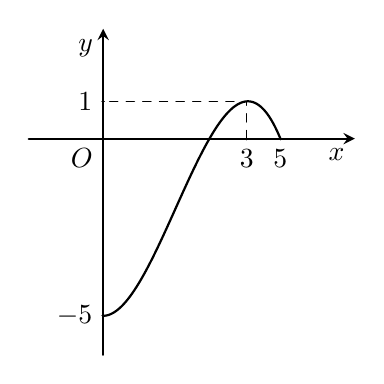
\begin{tikzpicture}[scale=0.45,line join=round, line cap=round,>=stealth,thick]
			\tikzset{every node/.style={scale=1}}
			\draw[->] (-2.1,0)--(7.1,0) node[below left] {$x$};
			\draw[->] (0,-6.1)--(0,3.1) node[below left] {$y$};
			\draw (0,0) node [below left] {$O$};
			\foreach \x/\nx in {4.05/3,5/5}
			\draw[thin] (\x,1pt)--(\x,-1pt) node [below] {$\nx$};
			\foreach \y/\ny in {-5/-5,1.05/1}
			\draw[thin] (1pt,\y)--(-1pt,\y) node [left] {$\ny$};
			\draw[dashed,thin](4.05,0)--(4.05,1.05)--(0,1.05);
			\begin{scope}
				\clip (-2,-6) rectangle (7,3);
				\draw[samples=200,domain=0:5,smooth,variable=\x] plot (\x,{-8/45*((\x)^3)+49/45*((\x)^2)+0*(\x)+-5});
			\end{scope}
		\end{tikzpicture}}
	\loigiai{
		Xét đồ thị hàm số $f'(x)$ trên đoạn $[0;5]$
		ta có $f'(x)=0\Leftrightarrow \hoac{& x=a\in (0;3) \\
				& x=5.}$\\
		Khi đó ta có bảng biến thiên của hàm số $y=f(x)$ như sau
		\begin{center}
			
\begin{tikzpicture}
				\tkzTabInit[nocadre=false,lgt=2,espcl=3,deltacl=0.9]
				{$x$/0.7,$P'(x)$/0.7,$P(x)$/1.5}{$0$,$a$,$5$}
				\tkzTabLine{,-,0,+,}
				\tkzTabVar{+/$f(0)$,-/$f(a)$,+/$f(5)$}
			\end{tikzpicture}
		\end{center}
		Ta có $a<3<5$ mà hàm số đồng biến trên $(a;5)$ nên $f(a)<f(3)<f(5)$.\\
		Gọi $S_1$ là phần hình phẳng giới hạn bởi các đường $y=f'(x)$, $Ox$, $x=0$, $x=a$.\\
		Gọi $S_2$ là phần hình phẳng giới hạn bởi các đường $y=f'(x)$, $Ox$, $x=0$, $x=5$.\\
		Ta có $\heva{&S_1=\displaystyle\int_0^a |f'(x)|\mathrm{\,d}x= f(0)-f(a)\\&S_2=\displaystyle\int_a^5 |f'(x)|\mathrm{\,d}x=f(5) -f(a).}$\\
		Mà $S_1>S_2\Leftrightarrow f(0)-f(a)>f(5)-f(a)\Leftrightarrow f(0)>f(5)$.\\
		Vậy $f(3)<f(5)<f(0)$.
	}
\end{ex} 
% \Closesolutionfile{ans}
% \Closesolutionfile{ansbook}

\cauds
% \Opensolutionfile{ansbook}[Ansbook/TenFile-TF]%---Nên đặt tên theo bài
% \setcounter{ex}{0}
\begin{ex}%[2D4C2-6]%[Dự án C đợt 3 - KSCL LeThanhTong-Võ Hoàng Nghĩa]
	Trong một cuộc thử tên lửa, Triều Tiên đã cho phóng một quả tên lửa có gắn đầu đạn hạt nhân với vận tốc $v(t) = \dfrac{1}{90\,000\,000}t^3 + \dfrac{1}{500}t + 1$ (m/s) trong đó $t$ đơn vị giây tính từ lúc tên lửa Triều Tiên bắt đầu phóng và dự định sẽ rơi xuống một vùng biển. Đi được $1$ giờ thì bay ngang vùng biển thuộc chủ quyền của Nhật Bản ngay lập tức Rada nhận được tín hiệu và gửi tín hiệu về căn cứ quân đội. Khi nhận được tín hiệu của Rada sau $30$ phút quân đội Nhật Bản đã cho phóng một quả tên lửa tầm trung đã xác định sẵn mục tiêu đi với gia tốc $a(t_1) = \dfrac{1}{4\,500}t_1 + \dfrac{n}{100}$ (m/s$^2$), $n > 0$ trong đó $t_1$ đơn vị giây tính từ lúc tên lửa tầm trung bắt đầu phóng.
	\choiceTF
	{Vận tốc của tên lửa tầm trung được biểu thị dưới hàm $v(t_1) = \dfrac{1}{9\,000}t_1^2 + \dfrac{n}{100}t_1$ (m/s$^2$), $n > 0$}
	{\True Kể từ khi bị Rada phát hiện đến lúc Nhật Bản phóng tên lửa thì quả tên lửa gắn đầu đạn hạt nhân đi được $1913{,}4$ km}
	{\True Sau $15$ phút phóng lên thì tên lửa tầm trung hạ được mục tiêu biết quãng đường nó đi được bằng $\dfrac{1}{2}$ quãng đường tên lửa Triều Tiên đi được trong $15$ phút đó, khi đó giá trị $n > 100$}
	{\True Giả sử hàm $h(t) = \dfrac{-5m}{648}t^2 + \dfrac{500m}{9}t + a$ $(m > 0, a \in \mathbb{R})$ (đơn vị: mét) thể hiện độ cao của quả tên lửa gắn đầu đạn hạt nhân so với mực nước biển. Khi quả tên lửa của Triều Tiên đạt độ cao lớn nhất thì quãng đường nó đi được là $483{,}12$ km}
	\loigiai{
		\begin{itemchoice}
			\itemch Vận tốc của tên lửa tầm trung được biểu thị dưới dạng hàm số như sau $$v(t_1)=\displaystyle\int{a(t_1)\mathrm{\,d}t_1}=\displaystyle\int{\left(\dfrac{1}{4500}t_1+\dfrac{n}{100} \right)\mathrm{\,d}t_1}=\dfrac{1}{9000}t_1^2+\dfrac{n}{100}t_1. \mathrm{(m/s)}$$
			\itemch Đổi $1$ giờ $= 3600$ giây và $1$ giờ $30$ phút $= 5400$ giây.\\
			Kể từ khi bị Rada phát hiện đến lúc Nhật Bản phóng tên lửa thì quả tên lửa gắn đầu đạn hạt nhân đi được là
			$$\displaystyle\int\limits_{3\,600}^{5\,400}{v(t)\mathrm{\,d}t}=\displaystyle\int\limits_{3\,600}^{5\,400}{\left(\dfrac{1}{90\,000\,000}t^3+\dfrac{1}{500}t+1 \right)\mathrm{\,d}t}=1\,913\,400\text{ (m)}=1\,913{,}4\text{ (km)}.$$
			\itemch Quãng đường tên lửa Triều Tiên đi được trong $15$ phút trước khi bị hạ là
			\[{s_{TT}}=\int\limits_{5\,400}^{6\,300}{\left(\dfrac{1}{90\,000\,000}t^3+\dfrac{1}{500}t+1 \right)\mathrm{\,d}t}=2\,025\,292{,}5 \text{ (m)}.\]
			Vì trong 15 phút đó, quãng đường tên lửa tầm trung đi được bằng $\dfrac{1}{2}$ quãng đường tên lửa Triều Tiên đi được, ta có
			\allowdisplaybreaks
			\begin{eqnarray*}
				&& s_{NB}=\dfrac{1}{2}s_{TT} \\
				&\Rightarrow& s_{NB}=1\,012\,646{,}25 \text{ (m)}\\
				&\Rightarrow& \displaystyle\int_0^{900} v(t_1)\mathrm{\,d}t_1 =1\,012\,646{,}25\\
				&\Rightarrow& \displaystyle\int_0^{900} \left( \dfrac{1}{9\,000}t_1^2+\dfrac{n}{100}t_1\right) \mathrm{\,d}t_1 =1\,012\,646{,}25\\
				&\Rightarrow& 27\,000+40\,500\cdot\dfrac{n}{100} =1\,012\,646{,}25\\
				&\Rightarrow& n \approx234{,}4>100.
			\end{eqnarray*}
			\itemch Khi quả tên lửa của Triều Tiên đạt độ cao lớn nhất thì
			\begin{eqnarray*}
				&& h'(t)=0 \\
				&\Leftrightarrow& -\dfrac{5m}{324}t+\dfrac{500m}{9}=0\\
				&\Leftrightarrow& t=3\,600.
			\end{eqnarray*}
			Khi quả tên lửa của Triều Tiên đạt độ cao lớn nhất thì quãng đường nó đi được là
			\[{s_{TT}}=\displaystyle\int\limits_0^{3600}{\left( \dfrac{1}{90\,000\,000}t^3+\dfrac{1}{500}t+1 \right)\mathrm{\,d}t}=483\,120\text{ (m)}=483{,}12 \text{ (km).}\]
		\end{itemchoice}
	}
\end{ex}

\begin{ex}%[2D1V4-3]%[Dự án C đợt 3 - KSCL LeThanhTong-Võ Hoàng Nghĩa]
	Cho hàm số $f(x)=\dfrac{x^{3}}{3}-3x-6\ln(2-x)+1$.
	\choiceTF
	{\True Đạo hàm của hàm số đã cho là $f'(x)=\dfrac{x^{3}-2x^{2}-3x}{x-2}$}
	{\True Hàm số đã cho đồng biến trong khoảng $(-\infty;-1)$}
	{\True Tổng các giá trị cực đại và cực tiểu của đồ thị hàm số bằng $\dfrac{14}{3}-6\ln(6)$}
	{Hàm số $g(x)=\dfrac{f(x)}{x^{2}+2x+2}$ có đường tiệm cận xiên có dạng $y=ax+b$. Khi đó $a+b=\dfrac{1}{3}$}
	\loigiai{
		\begin{itemchoice}
			\itemch Hàm số xác định trên khoảng $(-\infty;2)$ và
			$f'(x)=x^2-3+\dfrac{6}{2-x}=\dfrac{x^3-2x^2-3x}{x-2}$.
			\itemch Giải $f'(x)=0\Leftrightarrow x^3-2x^2-3x=0\Leftrightarrow\hoac{&x=3\\&x=-1\\&x=0.}$\\
			Bảng biến thiên
			\begin{center}
				
\begin{tikzpicture}
					\tkzTabInit
					[lgt=2,espcl=3.5] % tùy chọn lgt độ dọc/ espcl độ dài 
					{$x$/1.2, $f’(x)$/1, $f(x)$/2.5} % cột đầu tiên
					{$-\infty$, $-1$,$0$, $2$,$ $} % hàng 1 cột 2
					\tkzTabLine{,+,0,-,0,+,d,} % hàng 2 cột 2
					\tkzTabVar{-/$-\infty$,+/$\frac{11}{3}-6\ln 3$,-/$1-6\ln2$,+D/$+\infty$} % hàng 3 cột 2
				\end{tikzpicture}
			\end{center}
			Hàm số đã cho đồng biến trong khoảng $(-\infty;-1)$.
			\itemch Ta có $y_\text{CĐ}=y(-1)=\dfrac{11}{3}-6\ln 3$; $y_\text{CT}=y(0)=1-6\ln 2$. \\
			Suy ra $y_\text{CĐ}+y_\text{CT}=\dfrac{11}{3}-6\ln 3+1-6\ln 2=\dfrac{14}{3}-6\ln 6$.
			\itemch Xét $g(x)=\dfrac{f(x)}{x^{2}+2x+2}$ có đường tiệm cận xiên có dạng $y=ax+b$.\\
			Ta có $a=\lim\limits_{x\to-\infty}\dfrac{g(x)}{x}=\lim\limits_{x\to-\infty}\dfrac{\dfrac{x^3}{3}-3x-6\ln (2-x)+1}{x^3+2x^2+2x}=\dfrac{1}{3}$.\\ $b=\lim\limits_{x\to-\infty}\left(g(x)-\dfrac{1}{3}x \right)=\lim\limits_{x\to-\infty}\left(\dfrac{\dfrac{x^3}{3}-3x-6\ln (2-x)+1}{x^2+2x+2}-\frac{1}{3}x \right)=-\dfrac{2}{3}$. \\
			Vậy $a+b=\dfrac{1}{3}-\dfrac{2}{3}=-\dfrac{1}{3}$.
		\end{itemchoice}
	}
\end{ex}

\begin{ex}%[2H5C3-4]%[Dự án C đợt 3 - KSCL LeThanhTong-Võ Hoàng Nghĩa]
	Trong một cuộc thi thể thao về môn bắn súng. Các vận động viên phải thực hiện bắn hạ mục tiêu đang di động trên mặt của khối cầu đặc có bán kính bằng $1$ m. Chọn hệ trục tọa độ $(Oxyz)$ trong không gian có gốc $O$ đặt tại vị trí xạ thủ $A$ ngắm bắn, xem mặt phẳng $(Oxy)$ là mặt đất, đơn vị độ dài trên mỗi trục tọa độ là $1$ m. Biết khối cầu có tâm $I(7;24;3)$ và xem đường đi của viên đạn là một đường thẳng.
	\choiceTF
	{\True Vị trí xa nhất để xạ thủ $A$ nhìn thấy và ngắm bắn mục tiêu là $25,2$ m (làm tròn đến hàng phần mười)}
	{\True Biết vận tốc viên đạn là $\dfrac{54}{5}\sqrt{65}$ km/h thì khoảng thời gian ngắn nhất để xạ thủ $A$ bắn trúng mục tiêu chưa tới $1$ giây}
	{\True Để các xạ thủ có thể dễ dàng bắn trúng mục tiêu hơn, ban tổ chức đã quyết định cho mục tiêu di chuyển trên đường tròn lớn nhất của mặt cầu và song song với mặt đất. Khi đó khoảng cách ngắn nhất từ vị trí xạ thủ $A$ ngắm bắn đến mục tiêu là $3\sqrt{65}$ m}
	{\True Xạ thủ $A$ đang ngắm ở vị trí gần mục tiêu nhất. Tại thời điểm tuyển thủ $A$ nổ súng thì mục tiêu đang ở vị trí $M(6;24;3)$ di chuyển với vận tốc $v=\arctan\left(\dfrac{24}{7}\right)$ (m/s) và đi ngược chiều kim đồng hồ. Khi đó xạ thủ $A$ bắn trúng mục tiêu}
	\loigiai{\begin{center}
			\begin{tikzpicture}[line join=round, line cap=round,thick]
				%Gọi điểm
				\path
				(3,10) coordinate (I)
				($(I)-(3,0)$) coordinate (M)
				($(I)-(0.3,0.8)$) coordinate (N)
				($(I)+(2,2.25)$) coordinate (E)
				($(I)-(2.12,2.12)$) coordinate (F)
				($(I)-(-1.3,2.7)$) coordinate (T)
				(3,1) coordinate (H)
				(-5,9) coordinate (K)
				(-6,3) coordinate (A)
				(11,3) coordinate (B)
				(-11,0) coordinate (D)
				($ (B)+(D)-(A) $) coordinate (C)
				(-5,2) coordinate (O)
				;
				%Vẽ elip
				\draw[dashed,thin]
				(M) arc (180:0:3 cm and 0.8 cm)
				;
				%Vẽ đường tròn
				\draw
				(I) circle (3 cm)
				(M) arc (-180:0:3 cm and 0.8 cm)
				;
				%Vẽ mặt phẳng
				\draw (A)--(B)--(C)--(D)--cycle
				;
				%Vẽ hệ trục Oxyz
				\draw[->] (O)--(-8,0.3)node[left]{$ x $};
				\draw[->] (O)--(-1,2)node[below]{$ y $};
				%Nối hình chiếu
				\draw
				(I)--(O)
				(N)--(O)
				(T)--(O)
				(K)--(O)
				;
				\draw[dashed]
				(I)--(K)
				(I)--(H)
				(I)--(T)
				(I)--(E)
				;
				\node at ($ (I)+(1.1,0.05) $) {$ (7,24,3) $};
				\node at ($ (H)+(0.8,-0.35) $) {$ (7,24,0) $};
				\node at ($ (K)+(0.7,0.3) $) {$ (0,0,3) $};
				\foreach \i/\g in {O/-90,I/0,N/-90,F/180,T/0,K/90,H/-90}{\draw[fill=white](\i) circle (1.5pt) ($(\i)+(\g:3.3mm)$) node[scale=1]{$\i$};}
			\end{tikzpicture}
		\end{center}
		\begin{itemchoice}
			\itemch  Điểm xa nhất mà xạ thủ $A$ thấy được là tiếp điểm $B$ của tiếp tuyến kẻ từ $O$ đến mặt cầu.\\
			Ta có $OB^2=OI^2-IB^2=7^2+{{24}^2}+3^2-1^2\Rightarrow OB=\sqrt{633}\approx 25{,}2$ (m).
			\itemch Vì vận tốc không đổi nên khoảng thời gian ngắn nhất để xạ thủ $A$ bắn trúng mục tiêu là khoảng thời gian cho quãng đường từ xạ thủ đến vị trí gần xạ thủ nhất.\\
			Ta có $OC=OI-R=\sqrt{7^2+{{24}^2}+3^2}-1=\sqrt{634}-1$ (m).\\
			$v=\dfrac{54}{5}\sqrt{65}$ (km/h) $=3\sqrt{65}$ (m/s).\\
			Mặt khác, $t=\dfrac{s}{v}=\dfrac{OC}{v}=\dfrac{\sqrt{634}-1}{3\sqrt{65}}\approx 0{,}99969<1$ giây.
			\itemch
			Gọi $H(7;24;0)$ là hình chiếu của $I$ lên mặt phẳng $(Oxy)$. Vì đường tròn lớn nhất của mặt cầu nằm trong mặt phẳng song song với mặt đất nên khoảng cách ngắn nhất là $OD$ với $D$ là một trong hai giao điểm của mặt cầu, mặt phẳng $z=3$ và mặt phẳng $(OIH)$.\\
			Ta có $ID=1$; $OI=\sqrt{634}-1$; $\cos \widehat{DIO}=\cos \widehat{IOH}=\cos (\overrightarrow{OH},\overrightarrow{OI})=\dfrac{\sqrt{7^2+{{24}^2}}}{\sqrt{7^2+{{24}^2}+3^2}}=\dfrac{25}{\sqrt{634}}$.\\
			Suy ra $OD=\sqrt{OI^2+ID^2-2OI\cdot ID\cdot\cos \widehat{DOI}}=\sqrt{634+1-2\sqrt{634}.1.\dfrac{25}{\sqrt{634}}}=3\sqrt{65}$ (m).

			\itemch
			Ta có $\overrightarrow{IM}=(-1;0;0)$, $\overrightarrow{IO}=(-7;-24;-3)\Rightarrow \widehat{MIC}=(\overrightarrow{IM},\,\overrightarrow{IO})=\arccos \left(\dfrac{-1\cdot(-7)}{1\cdot\sqrt{634}} \right)=\arccos \left(\dfrac{7}{\sqrt{634}} \right)$.\\
			Khi đó, thời gian mục tiêu di chuyển từ $M$ đến điểm $C$ là \[{t_{mt}}=\dfrac{1\cdot\arccos \left(\dfrac{7}{\sqrt{634}} \right)}{\arctan \left( \dfrac{24}{7} \right) }\approx 1{,}0016 \text{ (giây)}.\]
			Thời gian viên đạn bay đến $C$ là ${t_{vd}}=\dfrac{OC}{v}=\dfrac{\sqrt{634}-1}{3\sqrt{65}}\approx 0{,}99969$ giây.
		\end{itemchoice}
	}
\end{ex}

\begin{ex}%[0D0V2-9]%[Dự án C đợt 3 - KSCL LeThanhTong-Võ Hoàng Nghĩa]
	Sau khi học kì I năm học 2024-2025, thầy Nghĩa chủ nhiệm lớp 12B5 nhận thấy rằng lớp mình có $60\%$ học sinh có kết quả xuất sắc, $40\%$ học sinh có kết quả loại giỏi, không có học sinh khá và trung bình. Nhưng để nắm bắt chính xác hơn về năng lực tư duy môn toán của từng học sinh nên thầy Nghĩa đã cho học sinh làm bài kiểm tra toán trong $90$ phút. Sau khi chấm bài xong, thầy Nghĩa thấy rằng trong số học sinh loại giỏi có $8$ học sinh từ $9$ điểm toán trở lên và có $75\%$ học sinh xuất sắc trong các học sinh được điểm toán từ 9 trở lên. Biết lớp 12B5 có $40$ học sinh.
	\choiceTF
	{\True Tỉ lệ học sinh có điểm toán từ $9$ trở lên của lớp 12B5 là $80\%$}
	{\True Học sinh xuất sắc kiểm tra môn toán đều lớn hơn hoặc bằng $9$ điểm}
	{\True Những học sinh có điểm toán dưới $9$ điểm đều là học sinh loại giỏi}
	{\True Có $22$ học sinh kết quả xuất sắc có điểm trên $9$ biết rằng tỉ lệ học sinh có điểm toán trên $9$ điểm của học sinh giỏi bằng $37{,}5\%$ và trong số học sinh có điểm bằng $9$ có $50\%$ học sinh xuất sắc}
	\loigiai{Số học sinh xuất sắc là $60\%\cdot40=24$ (học sinh).\\
		Số học sinh giỏi là $40\%\cdot40=16$ (học sinh).
		\begin{itemchoice}
			\itemch Gọi $x$ (học sinh) là số học sinh đạt từ $9$ điểm trở lên trong các học sinh xuất sắc $(0\le x\le 24)$.\\
			Số học sinh đạt từ $9$ điểm trở lên là $x+8$ (học sinh).\\
			Theo đề bài, ta có phương trình $\dfrac{x}{x+8}\cdot100\%=75\%\Leftrightarrow x=24$.\\
			Tỉ lệ học sinh có điểm toán từ $9$ điểm trở lên của lớp 12B5 là $\dfrac{24+8}{40}\cdot100\%=80\%$.
			\itemch Theo câu a ta có số học sinh xuất sắc từ $9$ điểm trở lên là $24$ học sinh và bằng tổng số học sinh xuất sắc.
			\itemch Từ câu a ta có số học sinh dưới $9$ điểm đều là học sinh giỏi và bằng $40-(24+8)=8$ (học sinh).
			\itemch Số học sinh giỏi có điểm trên $9$ là $16\cdot37{,}5\%=6$ (học sinh).\\
			Số học sinh giỏi có điểm bằng $9$ là $8-6=2$ (học sinh).\\
			Do trong số học sinh có điểm bằng $9$ có $50\%$ học sinh xuất sắc nên số học sinh xuất sắc có điểm bằng $9$ là $2$ (bằng số học sinh giỏi có điểm bằng $9$).
		\end{itemchoice}
	}
\end{ex}
% \Closesolutionfile{ansbook}


\caukq
% \Opensolutionfile{ansbt}[Ansbook/TenFile-TLN]%---Nên đặt tên theo bài
% \setcounter{ex}{0}
\begin{ex}%[1H8V7-3]
	Cho khối chóp $S.ABCD$ có đáy là hình thoi cạnh $2$, $\widehat{ABC}=120^\circ$, $SB=2$. Mặt phẳng $(SAD)$ vuông góc với mặt đáy và cạnh bên $SA$ tạo với mặt đáy một góc $60^\circ$. Tính thể tích khối chóp $S.ABCD$.
	\shortans[]{$1$}
	\loigiai{
		\immini{
			Gọi $SH$ là đường cao của $\triangle SAD$. \\
			Ta có $\heva{&(SAD)\perp(ABCD)\\&(SAD)\cap (ABCD)=AD\\&SH\perp AD, SH \subset (SAD)} \Rightarrow SH \perp (ABCD)$.\\
			Khi đó $(SA, (ABCD))=\widehat{SAH}=60^\circ$. \\
			Đặt $x=SH$ thì $AH=\dfrac{x}{\sqrt 3}$. \\
			Xét $\triangle SHB$ vuông tại $H$, ta có
			$$BH=\sqrt{SB^2-SH^2}=\sqrt{4-x^2}.$$
			Xét $\triangle ABH$, có $\widehat{HAB}=60^\circ$ (vì $\widehat{ABC}=120^\circ$).
		}{
			\begin{tikzpicture}[>=stealth,line join=round,line cap=round,font=\footnotesize,scale=.8]
				\path
				(0,0) coordinate (D)
				(-3,-2) coordinate (A)
				(6,0) coordinate (C)
				($(C)+(A)-(D)$) coordinate (B)
				($(D)!.75!(A)$) coordinate (H)
				($(H)+(90:5)$) coordinate (S)
				($(D)!.5!(B)$) coordinate (O)
				%		($(D)!.5!(O)$) coordinate (I)
				%		($(D)!.5!(C)$) coordinate (K)
				%		($(C)!.5!(B)$) coordinate (P)
				;
				\draw (S)--(A)--(B)--(C)--(S)--(B);
				\draw[dashed]
				(S)--(D)--(A)--(C)--(D)--(B) (S)--(H)--(B)
				;
				\foreach \p/\g in {S/90, D/170, A/-90, C/0, B/-90,  O/-90, H/180}
				\draw[fill=black] (\p) circle (1pt) node[shift=(\g:2.5mm)] {$\p$};
			\end{tikzpicture}
		}
		Áp dụng định lí cô sin, ta được:
		\allowdisplaybreaks
		\begin{eqnarray*}
			&& BH^2=AH^2+AB^2-2\cdot AH\cdot AB\cdot \cos \widehat{HAB} \\
			&\Leftrightarrow& 4-x^2=\dfrac{x^2}{3}+4-2\cdot2\cdot\dfrac{x}{\sqrt 3}\cdot\cos 60^\circ \\
			&\Rightarrow& x=\dfrac{\sqrt 3}{2}
		\end{eqnarray*}
		Vậy $V_{S.ABCD}=\dfrac{1}{3}\cdot SH\cdot S_{ABCD}=\dfrac{1}{3}\cdot SH\cdot AB\cdot AD \cdot \sin 60^\circ = \dfrac{1}{3}\cdot\dfrac{\sqrt 3}{2}\cdot 2\cdot 2 \cdot \sin 60^\circ=1$.
	}
\end{ex}

\begin{ex}%[2D4C3-2]%[Dự án C đợt 3 - KSCL LeThanhTong-Võ Hoàng Nghĩa]
	Một nhóm các kĩ sư muốn xây dựng một cây cầu vòm dàn thép với giá đỡ dưới bằng thép cao cấp có hình dáng là một parabol nối từ 2 cột trụ $A$ và $B$ nằm bên dưới cây cầu. Biết hai cột trụ cách nhau $400$ m, khoảng cách từ trụ $A$ đến cây cầu là $50$ m và $AB$ song song với mặt đường.
	% \begin{center}
	% 	\includegraphics[scale=1]{images/KSCL-THPT-LeThanhTong-HCM-NH24-25}
	% \end{center}
	Gắn hệ trục $Oxy$ vào cây cầu với đơn vị trục tọa độ là $10$ m. Giá đỡ dưới bằng thép là đường cong parabol tạo với hai trục tọa độ các hình phẳng có diện tích $S_1$, $S_2$ như hình vẽ bên. Biết rằng $S_2-2S_1=\dfrac{2200}{21}$. Điểm cao nhất của giá đỡ dưới bằng thép cao cấp cách mặt đường cây cầu bao nhiêu mét? (làm tròn đến hàng phần mười)
	\begin{center}
		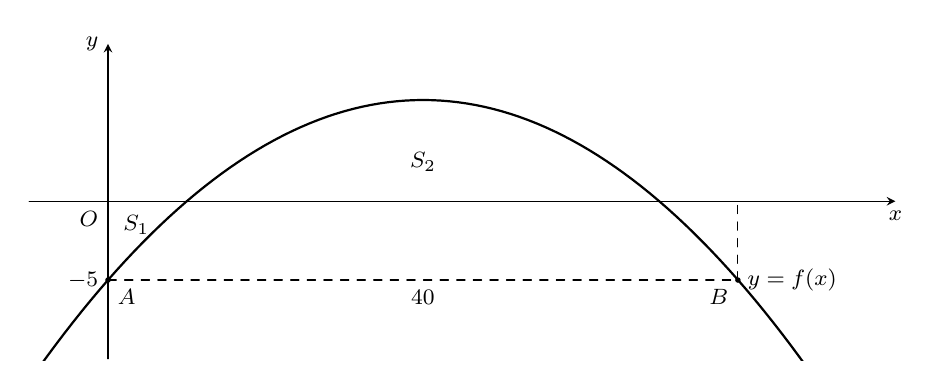
\begin{tikzpicture}[scale=1, font=\footnotesize, line join=round, line cap=round,>=stealth, xscale=0.2, yscale=0.2]
			%Gán số liệu.
			\def\xmin{-5};\def\ymin{-10};\def\xmax{50};\def\ymax{10};
			%Gán tọa độ.
			\coordinate (O) at (0,0);
			%Trục Oxy.
			\draw[->] (\xmin,0)--(\xmax,0) node[below]{$x$};
			\draw[->] (0,\ymin)--(0,\ymax) node[left]{$y$};
			\fill (O) node[below left]{$O$} circle(1pt);
			%Giới hạn đồ thị.
			\clip ({\xmin-0.1},{\ymin-0.1}) rectangle ({\xmax+0.1},{\ymax+0.1});
			%Vẽ đồ thị.
			\draw[thick,samples=100] plot[domain=-5:50](\x,{-1/35*(\x)^2+8/7*\x-5});
			\draw(40,-5) node[right]{$y=f(x)$};
			\draw [dashed] (40,-5)--(40,0);
			\draw [dashed] (0,-5)--(40,-5) node[midway,sloped,below]{$40$};
			\fill[fill=black](0,-5) node[left]{$-5$} circle(5pt);
			\fill[fill=black](40,-5) node[below left]{$B$} circle(5pt);
			\draw(0,-5) node [below right]{$A$};
			\draw(1.8,-1.5) node{$S_1$};
			\draw(20,2.5) node{$S_2$};
		\end{tikzpicture}
	\end{center}
	\shortans[]{$64{,}3$}
	\loigiai{
		\begin{center}
			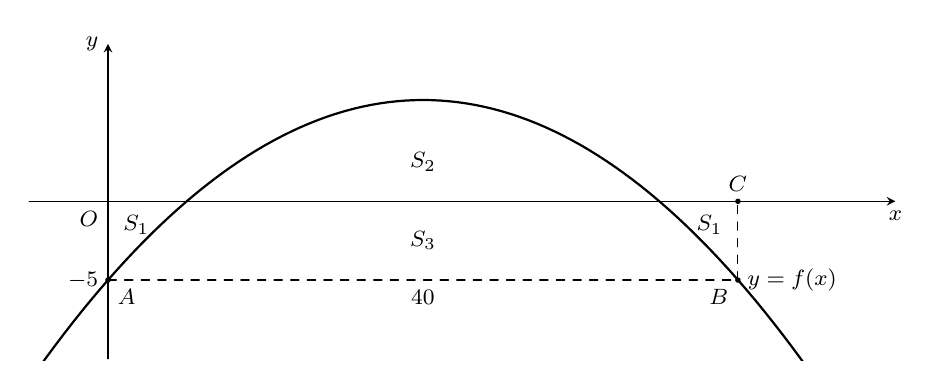
\begin{tikzpicture}[scale=1, font=\footnotesize, line join=round, line cap=round,>=stealth, xscale=0.2, yscale=0.2]
				%Gán số liệu.
				\def\xmin{-5};\def\ymin{-10};\def\xmax{50};\def\ymax{10};
				%Gán tọa độ.
				\coordinate (O) at (0,0);
				%Trục Oxy.
				\draw[->] (\xmin,0)--(\xmax,0) node[below]{$x$};
				\draw[->] (0,\ymin)--(0,\ymax) node[left]{$y$};
				\fill (O) node[below left]{$O$} circle(1pt);
				%Giới hạn đồ thị.
				\clip ({\xmin-0.1},{\ymin-0.1}) rectangle ({\xmax+0.1},{\ymax+0.1});
				%Vẽ đồ thị.
				\draw[thick,samples=100] plot[domain=-5:50](\x,{-1/35*(\x)^2+8/7*\x-5});
				\draw(40,-5) node[right]{$y=f(x)$};
				\draw [dashed] (40,-5)--(40,0);
				\draw [dashed] (0,-5)--(40,-5) node[midway,sloped,below]{$40$};
				\fill[fill=black](0,-5) node[left]{$-5$} circle(5pt);
				\fill[fill=black](40,-5) node[below left]{$B$} circle(5pt);
				\fill[fill=black](40,0) node[above]{$C$} circle(5pt);
				\draw(0,-5) node [below right]{$A$};
				\draw(1.8,-1.5) node{$S_1$};
				\draw(38.2,-1.5) node{$S_1$};
				\draw(20,2.5) node{$S_2$};
				\draw(20,-2.5) node{$S_3$};
			\end{tikzpicture}
		\end{center}
		Parabol có dạng $(P)\colon y=ax^2+bx+c$.\\
		Vì $(P)$ đi qua $(0;-5)$ nên $f(0)=-5 \Rightarrow c=-5$.\\
		Và $(P)$ đi qua $(40;-5)$ nên $f(40)=-5 \Rightarrow 1600a+40b+c=-5 \Rightarrow 1600a+40b=0 $. \hfill (1)\\
		Ta có
		\allowdisplaybreaks
		\begin{eqnarray*}
			S_2-2S_1 &=& S_2-(S_{OABC}-S_3)=(S_2+S_3)-S_{OABC}\\
			&=&\displaystyle\int_0^{40} \left( ax^2+bx+c+5\right) \mathrm{\,d}x-5\cdot40\\
			&=& \dfrac{64000}{3}a+800b+40c.
		\end{eqnarray*}
		Suy ra $\dfrac{64000}{3}a+800b +40c= \dfrac{6400}{21}$. \hfill $(2)$\\
		Từ $(1)$ và $(2)$ ta giải được $a=-\dfrac{1}{35}$, $b=\dfrac{8}{7}$. \\
		Suy ra $(P)\colon y=-\dfrac{1}{35}x^2+\dfrac{8}{7}x-5$.\\
		Do đó $(P)$ có đỉnh $I\left( 20;\dfrac{45}{7}\right) $.\\
		Vậy điểm cao nhất của giá đỡ dưới bằng thép cao cấp cách mặt đường cây cầu $10\cdot \dfrac{45}{7} \approx 64{,}3$ m.

	}
\end{ex}

\begin{ex}%[1H8V7-9]
	Cho khối trụ có bán kính là $R$ chiều cao $h$, hai đường tròn đáy có tâm là $O$ và $O'$. Một khối nón có đỉnh trùng với $O'$ và đáy có tâm $(O; 2R)$. Gọi $V_1$ là thể tích phần khối nón nằm bên ngoài khối trụ, $V_2$ là thể tích phần khối trụ nằm bên ngoài khối nón. Tính $\dfrac{V_1}{V_2}$?
	\shortans[]{2}
	\loigiai{
		\immini{
			\begin{itemize}
				\item Thể tích khối trụ chiều cao $h$ bán kính $R$ là
				      $V=\pi R^2 h.$
				\item Thể tích khối nón chiều cao $h$, bán kính $2R$ là % đỉnh $O'$, đường tròn đáy $(O;2R)$ là
				      $V_3=\dfrac{1}{3}\pi (2R)^2h=\dfrac{4}{3}V.$
				\item Thể tích khối nón chiều cao $\dfrac{h}{2}$, bán kính $R$ là
				      $V_4=\dfrac{1}{3}\pi R^2 \dfrac{h}{2}=\dfrac{1}{6}V.$
				\item Thể tích khối trụ chiều cao $\dfrac{h}{2}$, bán kính $R$ là
				      $V_5=\pi R^2 \dfrac{h}{2}=\dfrac{1}{2}V.$
				\item Thể tích hình nón cụt chiều cao $\dfrac{h}{2}$ và bán kính hai đáy lần lượt là $R$ và $2R$ là
				      $V_6=V_3-V_4=\dfrac{4}{3}V-\dfrac{1}{6}V=\dfrac{7}{6}V.$
			\end{itemize}
		}{
			\begin{tikzpicture}[scale=.7, font=\footnotesize, line join=round, line cap=round, >=stealth]
				\def\a{2} \def\b{0.5} \def\h{6}
				\path
				(0,0) coordinate (O)			(O)+(0,\h) coordinate (O')			(180:\a cm and \b cm) coordinate (A)			(A) + (0,\h) coordinate (B)
				(A) + (2*\a,0) coordinate (C)			(C) + (0,\h) coordinate (D)
				($(O)!2!(A)$) coordinate (A') ($(O)!2!(C)$) coordinate (C')
				($(B)!.5!(A)$) coordinate (M) ($(C)!.5!(D)$) coordinate (N)
				;
				\draw
				(O') ellipse (\a cm and \b cm)        %elip trên
				(A) arc (180:360:\a cm and \b cm) %elip dưới liền
				(M) arc (180:360:\a cm and \b cm) %elip dưới liền
				(A') arc (180:360:2*\a cm and 2*\b cm) %elip dưới liền
				(A)--(B) (C)--(D) (A')--(M) (C')--(N)
				;
				\draw[dashed]
				(A) arc (180:0:\a cm and \b cm)    %elip dưới đứt
				(M) arc (180:0:\a cm and \b cm)    %elip dưới đứt
				(A') arc (180:0:2*\a cm and 2*\b cm)    %elip dưới đứt
				(M)--(O')--(N)
				;
				\draw[dashed] (O')--(O)node[midway,left]{$h$}--(C) node[midway,above]{$R$};
				\foreach \p/\r in {O/180,O'/0}		\fill (\p) circle (1pt) node[shift={(\r:3mm)}]{$\p$};
			\end{tikzpicture}
		}
		\begin{itemize}
			\item Thể tích phần khối nón nằm bên ngoài khối trụ là
			      $V_1=V_6-V_5=\dfrac{7}{6}V-\dfrac{1}{2}V=\dfrac{2}{3}V$.
			\item Thể tích khối trụ bên ngoài khối nón là
			      $V_2=V_5-V_4=\dfrac{1}{2}V-\dfrac{1}{6}V=\dfrac{1}{3}V$.
			\item Vậy $\dfrac{V_1}{V_2}=2$.
		\end{itemize}
	}
\end{ex}

\begin{ex}%[2D1V3-2]%[Dự án C đợt 3 - KSCL LeThanhTong-Võ Hoàng Nghĩa]
	Anh Nam có một cái ao với diện tích $50$ m$^2$ để nuôi cá diêu hồng. Vụ vừa qua anh nuôi với mật độ $40$ con/m$^2$ và thu được $3$ tấn cá thành phẩm. Theo kinh nghiệm nuôi cá của mình anh thấy cứ thả giảm đi $8$ con/m$^2$ thì mỗi con cá thành phẩm thu được tăng thêm $0{,}5$ kg. Để tổng năng suất cao nhất thì vụ tới anh Nam nên mua bao nhiêu cá giống để thả? (giả sử không có hao hụt trong quá trình nuôi)
	\shortans[]{$1600$}
	\loigiai{
		Ở vụ trước.
		\begin{itemize}
			\item Số con cá được nuôi là $50\cdot40=2\,000$ con.
			\item Cân nặng trung bình mỗi con cá là $\dfrac{3\,000}{2\,000} =1{,}5$ kg.
		\end{itemize}
		Ở vụ này, giả sử anh Nam giảm $8x$ con cá trên một mét vuông. Khi đó
		\begin{itemize}
			\item Mật độ cá là $40-8x$ (con/m$^2$).
			\item Số con cá được nuôi là $50(40-8x)$.
			\item Khối lượng trung bình mỗi con cá là $1{,}5+0{,}5x$ kg.
			\item Tổng khối lượng (kg) cá thành phẩm là
			      $\begin{aligned}[t]
					      f(x) & =50(40-8x)(1{,}5+0{,}5x)  \\
					           & =-200x^2 + 400x + 3\,000.
				      \end{aligned}$
			\item[] Ta có $f'(x)=-400x+400$ và $f'(x)=0\Leftrightarrow x=1$.\\
			      Bảng biến thiên của hàm số $f(x)$ như sau
			      \begin{center}
				      
\begin{tikzpicture}
					      \tkzTabInit[nocadre=false,lgt=1.2,espcl=2.5,deltacl=0.6]
					      {$x$ /0.6,$f'(x)$ /0.6,$f(x)$ /2}
					      {,$1$,}
					      \tkzTabLine{,+,0,-,}
					      \tkzTabVar{-/,+/$3\,200$,-/}
				      \end{tikzpicture}
			      \end{center}
			      Dựa vào bảng biến thiên, ta thấy giá trị lớn nhất của $f(x)$ là $3\,200$ (kg) khi $x=1$.
		\end{itemize}
		Vậy để tổng năng suất của anh Nam ở vụ sau cao nhất thì vụ tới anh Nam số cá giống anh Nam nên mua để thả là $50(40-8\cdot1)=1600$ con cá.
	}
\end{ex}

\begin{ex}%[2H5C1-7]%[Dự án C đợt 3 - KSCL LeThanhTong-Võ Hoàng Nghĩa]
	\immini{
		Một cơ sở sản xuất Kem làm một mô hình Kem ốc quế lớn gồm 2 phần: Phần Kem có dạng hình cầu, phần ốc quế có dạng hình nón (như hình vẽ bên). Chủ cơ sở sản xuất muốn gắn một chiếc đèn Led lớn chiếu thẳng cây kem vào buổi tối, biết rằng chiếc đèn nằm trên mặt phẳng chứa đường tròn $(C)$ là phần tiếp xúc giữa phần Kem và phần ốc quế. Chọn hệ trục tọa độ $Oxy$ trong không gian thỏa mãn phần Kem hình cầu có tâm $I(1;2;3)$, bán kính $R_C=3$ và phần đỉnh của hình nón là điểm $H(0;1;-2)$ đáy là đường tròn có bán kính $R_N = \sqrt{6}$.
	}{
		\begin{tikzpicture}[line join = round, line cap = round, >=stealth, font=\footnotesize, scale=1]
			\tikzset{label style/.style={font=\footnotesize}}
			\def\r{1.5}

			\coordinate (I) at (0,0);
			\coordinate (a) at ($(I)+(-25:\r cm)$);
			\coordinate (b) at ($(I)+(-155:\r cm)$);
			\coordinate (a') at ($(a)!1!-90:(I)$);
			\coordinate (b') at ($(b)!1!-90:(I)$);
			\draw (intersection of  a--a' and b--b') coordinate (H);
			\draw (intersection of  I--H and a--b) coordinate (J);
			\draw[dashed] (a) arc (0:180:1.35cm and 0.35cm);
			\draw (a) arc (0:-180:1.35cm and 0.35cm);
			\draw[fill=black!20!white,opacity=0.5,draw=black] (I) circle (\r cm);
			\draw (a)--(H)--(b);
			\draw[fill=black!50!white, opacity=0.5] (a) arc (0:-180:1.35cm and 0.35cm)--(b)--(H)--(a)--cycle;
		\end{tikzpicture}
		\hspace{0.3cm}
		\begin{tikzpicture}[line join = round, line cap = round, >=stealth, font=\footnotesize, scale=1]
			\tikzset{label style/.style={font=\footnotesize}}
			\def\r{1.5}

			\coordinate[label={right}:{$I$}] (I) at (0,0);
			\coordinate (a) at ($(I)+(-25:\r cm)$);
			\coordinate (b) at ($(I)+(-155:\r cm)$);
			\coordinate (a') at ($(a)!1!-90:(I)$);
			\coordinate (b') at ($(b)!1!-90:(I)$);
			\draw (intersection of  a--a' and b--b') coordinate[label={right}:{$H$}] (H);
			\draw (intersection of  I--H and a--b) coordinate (J);
			\draw[dashed] (a) arc (0:180:1.35cm and 0.35cm);
			\draw (a) arc (0:-180:1.35cm and 0.35cm);
			\draw (I) circle (\r cm);
			\draw (a)--(H)--(b);
			\foreach \x in {I,H,J}
			\draw[fill=black] (\x) circle (1pt);
		\end{tikzpicture}
	}
	\noindent Để tối ưu hóa lượng ánh sáng chiếc đèn có thể chiếu vào cây kem người ta tính toán rằng chiếc đèn Led sẽ phải ở vị trí $M(a;b;2)$, $a\in \mathbb{Z}$ và từ điểm M kẻ được 2 tiếp tuyến với đường tròn $(C)$ sao cho góc giữa 2 tiếp tuyến đó không bé hơn $60^\circ$. Có bao nhiêu vị trí đặt chiếc đèn Led thỏa mãn yêu cầu của chủ cơ sở.
	\shortans{6}
	\loigiai{
	\immini{
		Ta có
		\allowdisplaybreaks
		\begin{eqnarray*}
			&& KI = \sqrt{R_C^2 - R_N^2} = \sqrt{3^2 - (\sqrt{6})^2} = \sqrt{3}.\\
			&& IH = \sqrt{(-1)^2 + (-1)^2 + (-5)^2} = 3\sqrt{3}.\\
			&\Rightarrow& \dfrac{IK}{IH} = \dfrac{1}{3} \\
			&\Rightarrow& \overrightarrow{IK} = \dfrac{1}{3}\overrightarrow{IH}
		\end{eqnarray*}
		Suy ra
		\[
			\heva{
				& x_K - 1 = -\dfrac{1}{3} \\
				& y_K - 2 = -\dfrac{1}{3} \\
				& z_K - 3 = -\dfrac{5}{3}
			}
			\Rightarrow
			\heva{
				&x_K = \dfrac{2}{3} \\
				&y_K = \dfrac{5}{3} \\
				&z_K = \dfrac{4}{3}
			}
			\Rightarrow K\left(\dfrac{2}{3};\dfrac{5}{3};\dfrac{4}{3}\right).
		\]
	}{
		\begin{tikzpicture}[line join = round, line cap = round, >=stealth, font=\footnotesize, scale=1]
			\tikzset{label style/.style={font=\footnotesize}}
			\def\r{1.5}

			\coordinate[label={right}:{$I$}] (I) at (0,0);
			\coordinate (a) at ($(I)+(-25:\r cm)$);
			\coordinate (b) at ($(I)+(-155:\r cm)$);
			\coordinate (a') at ($(a)!1!-90:(I)$);
			\coordinate (b') at ($(b)!1!-90:(I)$);
			\draw (intersection of  a--a' and b--b') coordinate[label={right}:{$H$}] (H);
			\draw (intersection of  I--H and a--b) coordinate[label={right}:{$K$}] (K);

			\coordinate[label={below}:{$B$}] (B) at ($(K)+(-110:1.35cm and 0.35cm)$);
			\coordinate[label={above}:{$A$}] (A) at ($(K)+(120:1.35cm and 0.35cm)$);
			\coordinate[label={left}:{$M$}] (M) at ($(K)!2.5!(b)$);

			\draw[dashed] (a) arc (0:180:1.35cm and 0.35cm);
			\draw (a) arc (0:-180:1.35cm and 0.35cm);
			\draw (I) circle (\r cm);
			\draw (a)--(H)--(b) (B)--(M)--(A) (M)--(b);
			\draw[dashed] (H)--(I) (b)--(K) (A)--(K)--(B);
			\foreach \x in {I,H,K,B,A,M}
			\draw[fill=black] (\x) circle (1pt);
		\end{tikzpicture}
	}
	Mặt phẳng $(MAB)$ đi qua $K$ và có VTPT là $\overrightarrow{IH} = (1; 1; 5)$ nên $(MAB)\colon x + y + 5z - 9 = 0$.\\
	Vì $M \in (MAB) \Rightarrow a + b + 5 \cdot 2 - 9 = 0 \Leftrightarrow b = -a - 1.$\\
	Khi đó
	$$KM = \sqrt{\left(a - \dfrac{2}{3}\right)^2 + \left(b - \dfrac{5}{3}\right)^2 + \left(2 - \dfrac{4}{3}\right)^2} = \sqrt{\left(a - \dfrac{2}{3}\right)^2 + \left(a + \dfrac{8}{3}\right)^2 + \left(2 - \dfrac{4}{3}\right)^2} = \sqrt{2a^2 + 4a + 8}.$$
	Và
	$$\widehat{AKM} = \dfrac{1}{2}\widehat{AKB} = \dfrac{1}{2} \left( 180^{\circ} - \widehat{AMB} \right) = 90^{\circ} - \dfrac{1}{2}\widehat{AMB} \le 90^{\circ} - \dfrac{1}{2} \cdot 60^{\circ} = 60^{\circ}.$$
			Vì $0^{\circ} < \widehat{AKM} \le 60^{\circ}$ nên $\dfrac{1}{2} \leq \cos \widehat{AKM} <1$. \hfill (1)\\
			Mặt khác $\cos \widehat{AKM} = \dfrac{KA}{KM} = \dfrac{\sqrt{6}}{\sqrt{2a^2 + 4a + 8}} = \sqrt{\dfrac{3}{a^2 + 2a + 4}}$. \hfill (2)\\
			Từ (1) và (2) suy ra $\dfrac{1}{2} \le \sqrt{\dfrac{3}{a^2 + 2a + 4}} < 1 \Leftrightarrow \dfrac{1}{4} \le \dfrac{3}{a^2 + 2a + 4} < 1 \Leftrightarrow 3 < a^2 + 2a + 4 \le 12$.\\
			Như vậy
			$$
				\heva{
					&a^2 + 2a - 8 \leq 0 \\
					&a^2 + 2a + 1 > 0
				} \Leftrightarrow
				\heva{
					&-4 \leq a \leq 2 \\
					&a \neq -1.
				}$$
			Vì $a \in \mathbb{Z}$ nên $a \in \{-4; -3; -2; 0; 1; 2\}$.\\
			Vậy có $6$ vị trí đặt đèn thỏa mãn.
		}
\end{ex}

\begin{ex}%[2D5C2-4]%[Dự án C đợt 3 - KSCL LeThanhTong-Võ Hoàng Nghĩa]
	Có hai hộp: hộp $I$ có $5$ quả bóng trắng và $7$ quả bóng đỏ, hộp $II$ có $10$ quả bóng trắng và $15$ quả bóng đỏ, các quả bóng có cùng kích thước và khối lượng. Lấy ngẫu nhiên hai quả bóng từ hộp $I$ bỏ vào hộp $II$. Sau đó, lấy ra ngẫu nhiên một quả bóng từ hộp $II$. Xác suất để quả bóng được lấy ra từ hộp $II$ là quả bóng được chuyển từ hộp $I$ sang, biết rằng quả bóng đó có màu trắng là $\dfrac{a}{b}$ (là phân số tối giản). Tính $a+b$.
	\shortans{14}
	\loigiai{
		Gọi $X$ là biến cố \lq\lq lấy được bóng trắng từ hộp $II$ sau khi đã chuyển $2$ bóng từ hộp $I$ sang\rq\rq.\\
		Gọi $Y$ là biến cố \lq\lq$2$ bóng được chuyển từ hộp $I$ sang hộp $II$\rq\rq.\\
		Ta có công thức Bayes: $\mathrm{P}(Y | X) = \dfrac{\mathrm{P}(X | Y) \cdot \mathrm{P}(Y)}{\mathrm{P}(X)}$. Trong đó:
		\begin{itemize}
			\item $\mathrm{P}(X | Y)$ là xác suất lấy được bóng trắng từ hộp $II$, biết rằng bóng đó được chuyển từ hộp $I$ sang.
			\item $\mathrm{P}(Y)$ là xác suất 2 bóng được chuyển từ hộp $I$ sang hộp $II$.
			\item $\mathrm{P}(X)$ là xác suất lấy được bóng trắng từ hộp $II$ sau khi chuyển $2$ bóng từ hộp $I$ sang.
		\end{itemize}
		Tính $\mathrm{P}(Y)$: Do ta không cần tính xác suất để $2$ bóng được chuyển từ hộp $I$ sang hộp $II$, biến cố này luôn xảy ra. Nên ta có thể bỏ qua yếu tố $\mathrm{P}(Y)$ trong công thức Bayes.\\
		Tính $\mathrm{P}(X)$: Có $3$ trường hợp xảy ra khi chuyển $2$ bóng từ hộp $I$ sang hộp $II$:
		\begin{itemize}
			\item TH1. Chuyển $2$ bóng trắng: Xác suất là $\dfrac{\mathrm{C}_{5}^{2}}{\mathrm{C}_{12}^{2}} = \dfrac{10}{66}$.
			      \begin{itemize}
				      \item Hộp $II$ có $12$ bóng trắng và $15$ bóng đỏ.
				      \item Xác suất lấy được bóng trắng từ hộp $II$ là $\dfrac{12}{27}$.
			      \end{itemize}
			\item TH2. Chuyển $1$ bóng trắng và $1$ bóng đỏ: Xác suất là $\dfrac{\mathrm{C}_{5}^{1} \cdot \mathrm{C}_{7}^{1}}{\mathrm{C}_{12}^{2}} = \dfrac{35}{66}$.
			      \begin{itemize}
				      \item Hộp $II$ có $11$ bóng trắng và $16$ bóng đỏ.
				      \item Xác suất lấy được bóng trắng từ hộp $II$ là $\dfrac{11}{27}$
			      \end{itemize}
			\item TH3. Chuyển $2$ bóng đỏ: Xác suất là $\dfrac{\mathrm{C}_{7}^{2}}{\mathrm{C}_{12}^{2}} = \dfrac{21}{66}$.
			      \begin{itemize}
				      \item Hộp $II$ có $10$ bóng trắng và $17$ bóng đỏ.
				      \item Xác suất lấy được bóng trắng từ hộp $II$ là $\dfrac{10}{27}$
			      \end{itemize}
		\end{itemize}
		Vậy, $\mathrm{P}(X) = \dfrac{10}{66} \cdot \dfrac{12}{27} + \dfrac{35}{66} \cdot \dfrac{11}{27} + \dfrac{21}{66} \cdot \dfrac{10}{27} = \dfrac{120 + 385 + 210}{66 \cdot 27} = \dfrac{715}{1782} = \dfrac{65}{162}$.\\
		Tính $\mathrm{P}(X|Y)$: Ta cần tính xác suất để bóng lấy ra từ hộp $II$ là bóng trắng được chuyển từ hộp $I$ sang.
		\begin{itemize}
			\item TH1. Trường hợp chuyển $2$ bóng trắng: Xác suất lấy được bóng trắng chuyển từ hộp $I$ là $\dfrac{2}{27}$.
			\item TH2. Trường hợp chuyển $1$ bóng trắng và $1$ bóng đỏ: Xác suất lấy được bóng trắng chuyển từ hộp $I$ là $\dfrac{1}{27}$.
			\item TH3. Trường hợp chuyển $2$ bóng đỏ: Xác suất lấy được bóng trắng chuyển từ hộp $I$ là $0$.
		\end{itemize}
		Vậy, $\mathrm{P}(X|Y) = \dfrac{10}{66} \cdot \dfrac{2}{27} + \dfrac{35}{66} \cdot \dfrac{1}{27} + \dfrac{21}{66} \cdot 0 = \dfrac{20 + 35}{66 \cdot 27} = \dfrac{55}{1782} = \dfrac{5}{162}$.\\
		Áp dụng công thức Bayes: $\mathrm{P}(Y|X) = \dfrac{\mathrm{P}(X|Y)}{\mathrm{P}(X)} = \dfrac{\dfrac{5}{162}}{\dfrac{65}{162}} = \dfrac{5}{65} = \dfrac{1}{13}$.\\
		Vậy $\dfrac{a}{b} = \dfrac{1}{13}$, suy ra $a = 1$ và $b = 13$. Suy ra $a + b = 1 + 13 = 14$.
	}
\end{ex}

\Closesolutionfile{ans}
\inputansbox{6,4,3}{ans/LeThanhTong}